\section{Przypadek Testowy 2 - Algorytm genetyczny - zależność PRD od wskaźnika mutacji}
  \subsection{Cel:}
    W tej części zostaną ze sobą porównane PRD rozwiązania algorytmu genetycznego w zależności od wskaźnika mutacji.
    \subsection{Założenia:}
    Do badania tego przypadku została wykorzystana instancje 
    \begin{itemize}
      \item berlin52.tsp
      \item eil76.tsp
      \item eil51.tsp
      \item gr17.tsp
      \item gr21.tsp
      \item gr24.tsp
      \item gr48.tsp
      \item hk48.tsp
      \item kroA100.tsp
      \item kroA150.tsp
      \item kroB100.tsp
      \item kroB150.tsp
      \item swiss42.tsp
      \item ftv33.atsp
      \item ftv35.atsp
      \item ftv38.atsp
      \item ftv44.atsp
      \item ftv47.atsp
      \item br17.atsp
    \end{itemize} 
    Dodatkowo współczynnik selekcji został ustalony na 0.7, wielkość populacji została ustalona na 100, liczba iteracji to 200. Badane współczynniki mutacji \(m \in {0.05, 0.10, 0.15 ... 0.95}\). Metoda selekcji to obcięcie.
  \subsection{Wyniki: }
  Poniższa tabela przedstawia wyniki testów, odchylenie standardowe oraz błęd standardowy.
  \begin{table}[!ht]
    \centering
    \begin{tabular}{|l|l|l|l|}
    \hline
        MR & PRD & SD & SE \\ \hline
        0.05 & 119.80 & 125.64 & 29.61 \\ \hline
        0.10 & 105.52 & 118.54 & 27.94 \\ \hline
        0.15 & 96.14 & 109.88 & 25.90 \\ \hline
        0.20 & 88.65 & 104.24 & 24.57 \\ \hline
        0.25 & 81.35 & 101.21 & 23.85 \\ \hline
        0.30 & 88.38 & 102.82 & 24.24 \\ \hline
        0.35 & 83.54 & 97.42 & 22.96 \\ \hline
        0.40 & 81.49 & 96.37 & 22.71 \\ \hline
        0.45 & 82.40 & 100.09 & 23.59 \\ \hline
        0.50 & 88.34 & 106.14 & 25.02 \\ \hline
        0.55 & 93.55 & 107.88 & 25.43 \\ \hline
        0.60 & 101.05 & 113.10 & 26.66 \\ \hline
        0.65 & 100.91 & 112.06 & 26.41 \\ \hline
        0.70 & 115.50 & 109.33 & 25.77 \\ \hline
        0.75 & 120.50 & 110.17 & 25.97 \\ \hline
        0.80 & 129.11 & 118.01 & 27.81 \\ \hline
        0.85 & 131.69 & 113.98 & 26.87 \\ \hline
        0.90 & 137.50 & 115.65 & 27.26 \\ \hline
        0.95 & 142.55 & 118.34 & 27.89 \\ \hline
    \caption{PRD - wyrażone w procętach [\%], SD - Odchylenie standardowe, SE - Błąd standardowy}
  \end{table}

  Odchylenie standardowe oraz błąd standardowy zostały obliczone według wzorów: \\
  Odchylenie standardowe:
  \[ \sigma = \sqrt{\frac{\sum_{n = 1}^{18}(\bar{x} - x_n)^2}{18}} \]
  Błąd standardowe:
  \[ \sigma_{\bar{x}} = \frac{\sigma}{\sqrt{18}} \]

  \subsection{Wykresy: }
    \begin{figure}[H]
      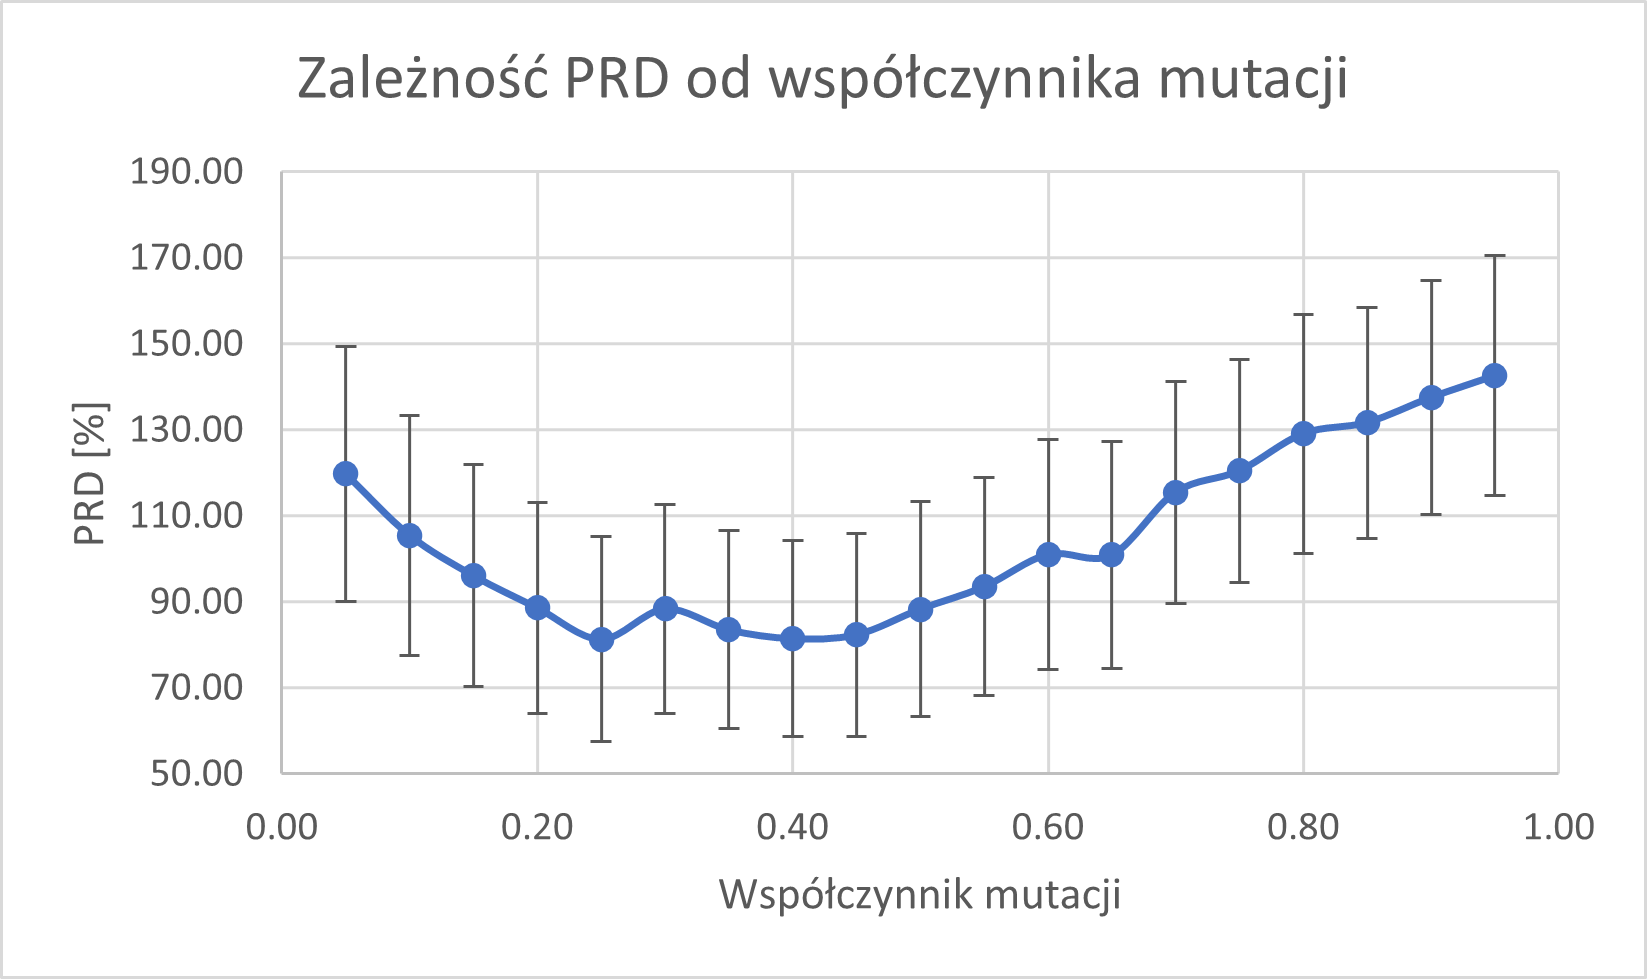
\includegraphics[scale=0.9]{chart_test_2.png}
      \centering
      \caption{zależność PRD od współczynnika mutacji}
    \end{figure}
  Na wykresach przedstawione są średnie wartości PRD dla badanych danych.

  \subsection{Wnioski: }
  Dla zebranych wyników, dla współczynnika mutacji w zakresie od 0.00 do 0.25 oraz 0.30 do 0.40 PRD maleje, od 0.4 do 1.00 rośnie. Przy szansie na mutację 0.25 algorytm osiągnął minimum w testach. Po przekroczeniu 0.5 algorytm daje coraz gorsze wyniki co ma związek z częstymi mutacjami - bardziej zaczyna przypominać k-random.

